\documentclass[12pt]{article}
\usepackage{amsmath,amssymb,latexsym}
\usepackage{graphicx,psfrag,epsf}
\usepackage{enumerate}
\usepackage{natbib}
\usepackage{wrapfig}
\usepackage{subcaption}

\newcommand{\blind}{0}

\addtolength{\oddsidemargin}{-.75in}%
\addtolength{\evensidemargin}{-.75in}%
\addtolength{\textwidth}{1.5in}%
\addtolength{\textheight}{1.3in}%
\addtolength{\topmargin}{-.8in}%
\pagenumbering{gobble}

\begin{document}
\pagenumbering{arabic}

%\bibliographystyle{natbib}

\def\spacingset#1{\renewcommand{\baselinestretch}%
{#1}\small\normalsize} \spacingset{1}


%%%%%%%%%%%%%%%%%%%%%%%%%%%%%%%%%%%%%%%%%%%%%%%%%%%%%%%%%%%%%%%%%%%%%%%%%%%%%%

\if0\blind
{
  \title{\bf Measuring the Electric Charge of Ping Pong Balls After Friction }
  \author{Stanley Zheng \quad Yuzhe Wang}
  \maketitle
} \fi

\if1\blind
{
  \bigskip
  \bigskip
  \bigskip
  \begin{center}
    {\LARGE\bf Title}
\end{center}
  \medskip
} \fi

\bigskip
\begin{abstract}
The purpose of this experiment is to measure the electric charge of a plastic ball. To construct our experiment, we used a long rope to tighten two small plastic balls respectively and measure the distance between the two balls. Then we compute the angle between the two ropes and use Coulomb's law to compute the consequence.
\end{abstract}


\spacingset{1.45}
\section{Introduction}
\label{sec:intro}

Electric charge is a fundamental property of matter that determines how it interacts with other matter and electromagnetic fields. Measuring the electric charge of an object or a system is important for many reasons, such as understanding the structure and behavior of atoms and molecules, designing and operating electrical devices and circuits, and studying the phenomena of electricity and magnetism. 

However, measuring the electric charge is not a trivial task, as it requires precise instruments and methods that can overcome the challenges posed by the quantum nature of charge and the influence of external factors such as electric fields and noise. In this article, we will use a fundamental and simple method to measure the electric charge of an object.


\section{Principle}


The principle of measuring the electric charge of a plastic ball using Coulomb's law is based on the idea that two charged objects exert a force on each other that is proportional to the product of their charges and inversely proportional to the square of the distance between them.

The experiment uses two small plastic balls, with a diameter of about 2 cm, a long rope, and a towel. The balls are attached to the ends of the rope and hung from a fixed point. The towel is used to rub the balls and transfer some electrons from one material to another, creating a net charge on each ball. The charged balls repel each other and move away from the vertical position, forming an angle with the rope. By measuring this angle and knowing the length of the rope and the mass of the balls, one can calculate the force acting on each ball and use Coulomb's law to estimate the charge on each ball.


\section{Experimental Procedure}

\begin{figure}[h]
    \centering
    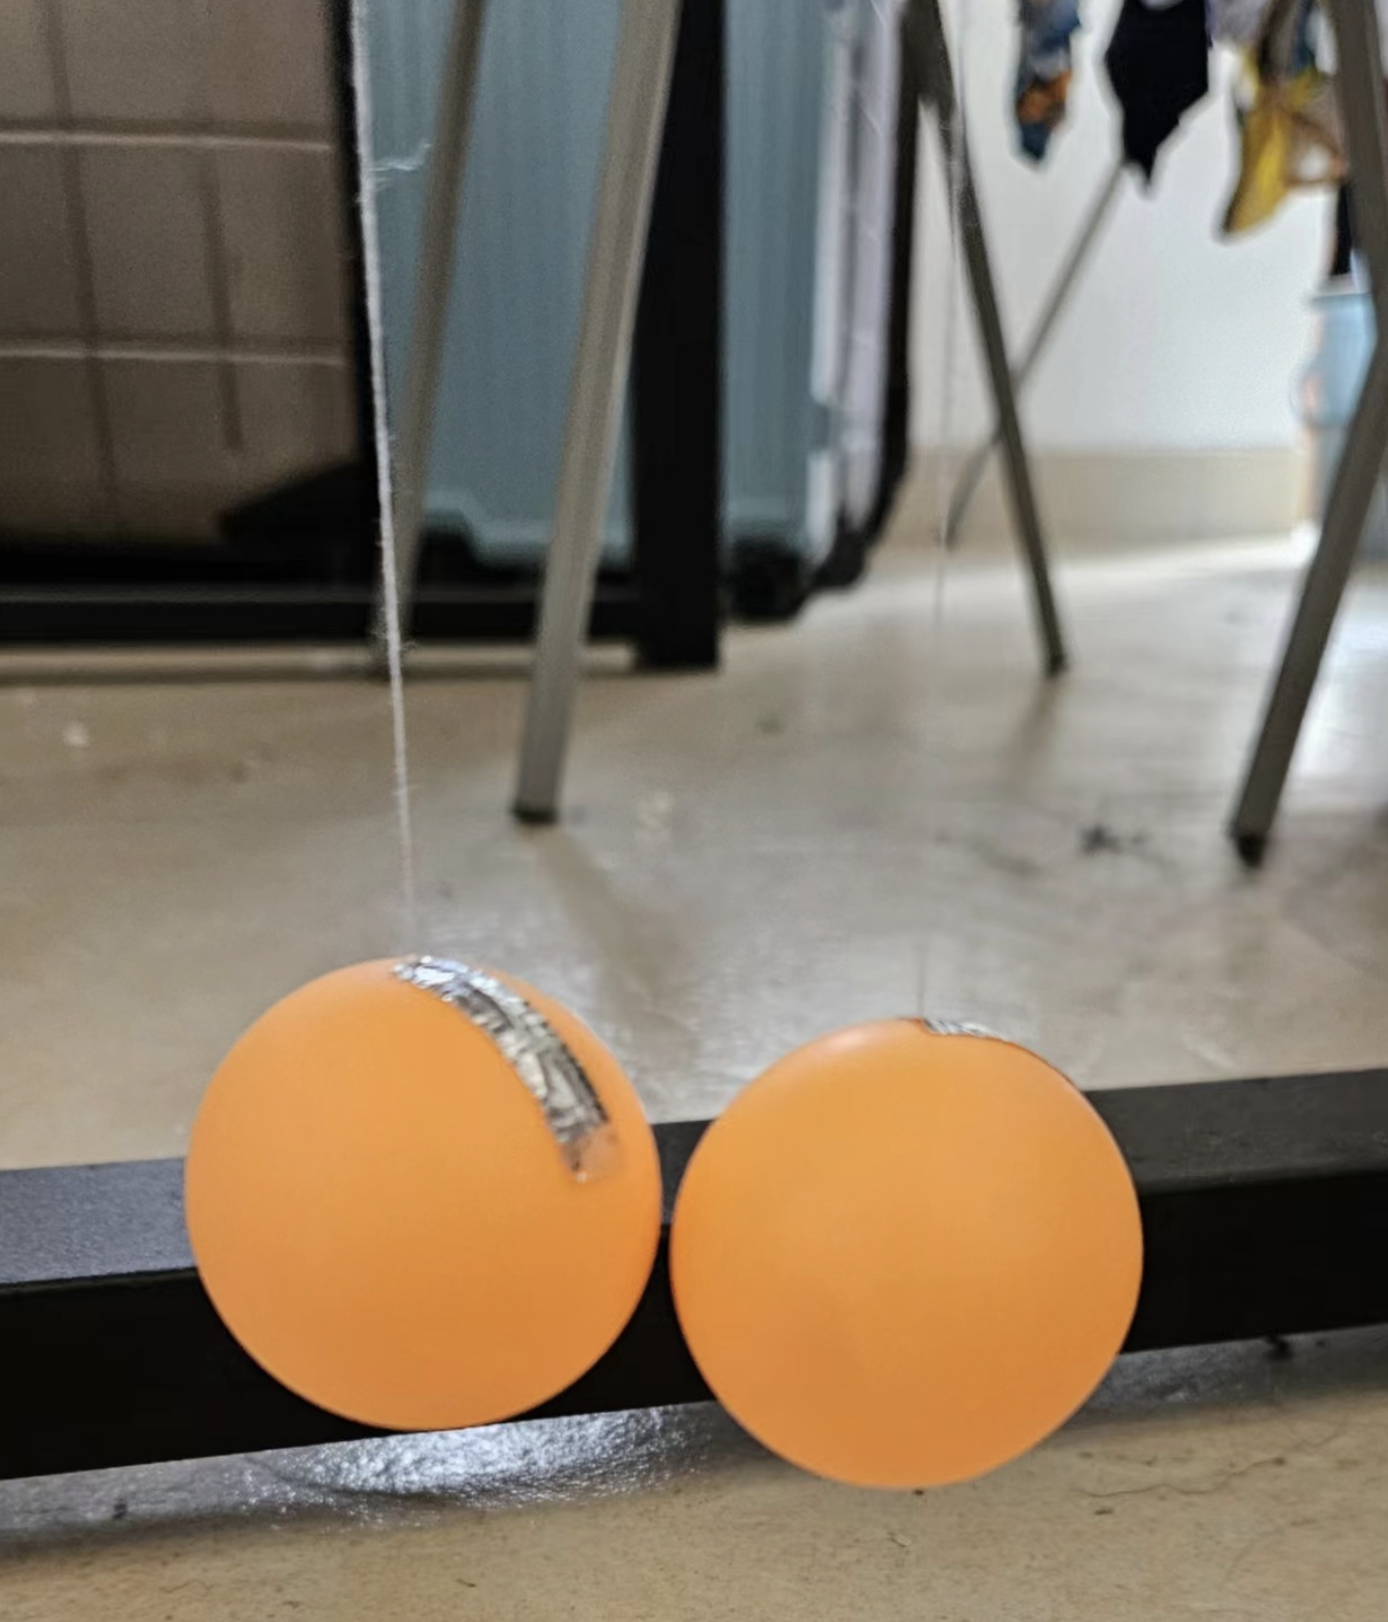
\includegraphics[width=0.4\linewidth]{1.png}
    \caption{The Separated Ping Pang Balls.}
\end{figure}

In the Figure 1, we first identified a platform created by combining a table and a camera tripod, achieving a height of 2 meters. This height was chosen to maximize the angular separation between two ping pong balls. Subsequently, we taped two ping pong balls together onto a single string and suspended them from the platform. The alignment of the two ping pong balls was adjusted to be on the same horizontal line, and the string was fixed in place.

Next, one of the ping pong balls was subjected to friction, and a small object was used to confirm the presence of a strong electric charge. The charged ping pong ball was then brought into contact with the other ping pong ball, ensuring that both balls acquired an equal amount of the same type of charge. The tension in the string was slowly released, allowing the two ping pong balls to come to rest, resulting in the formation of an angle, as depicted in the Figure 2.

\begin{figure}[htb]
\centering
\subfloat[Actual Structure Diagram.]{
		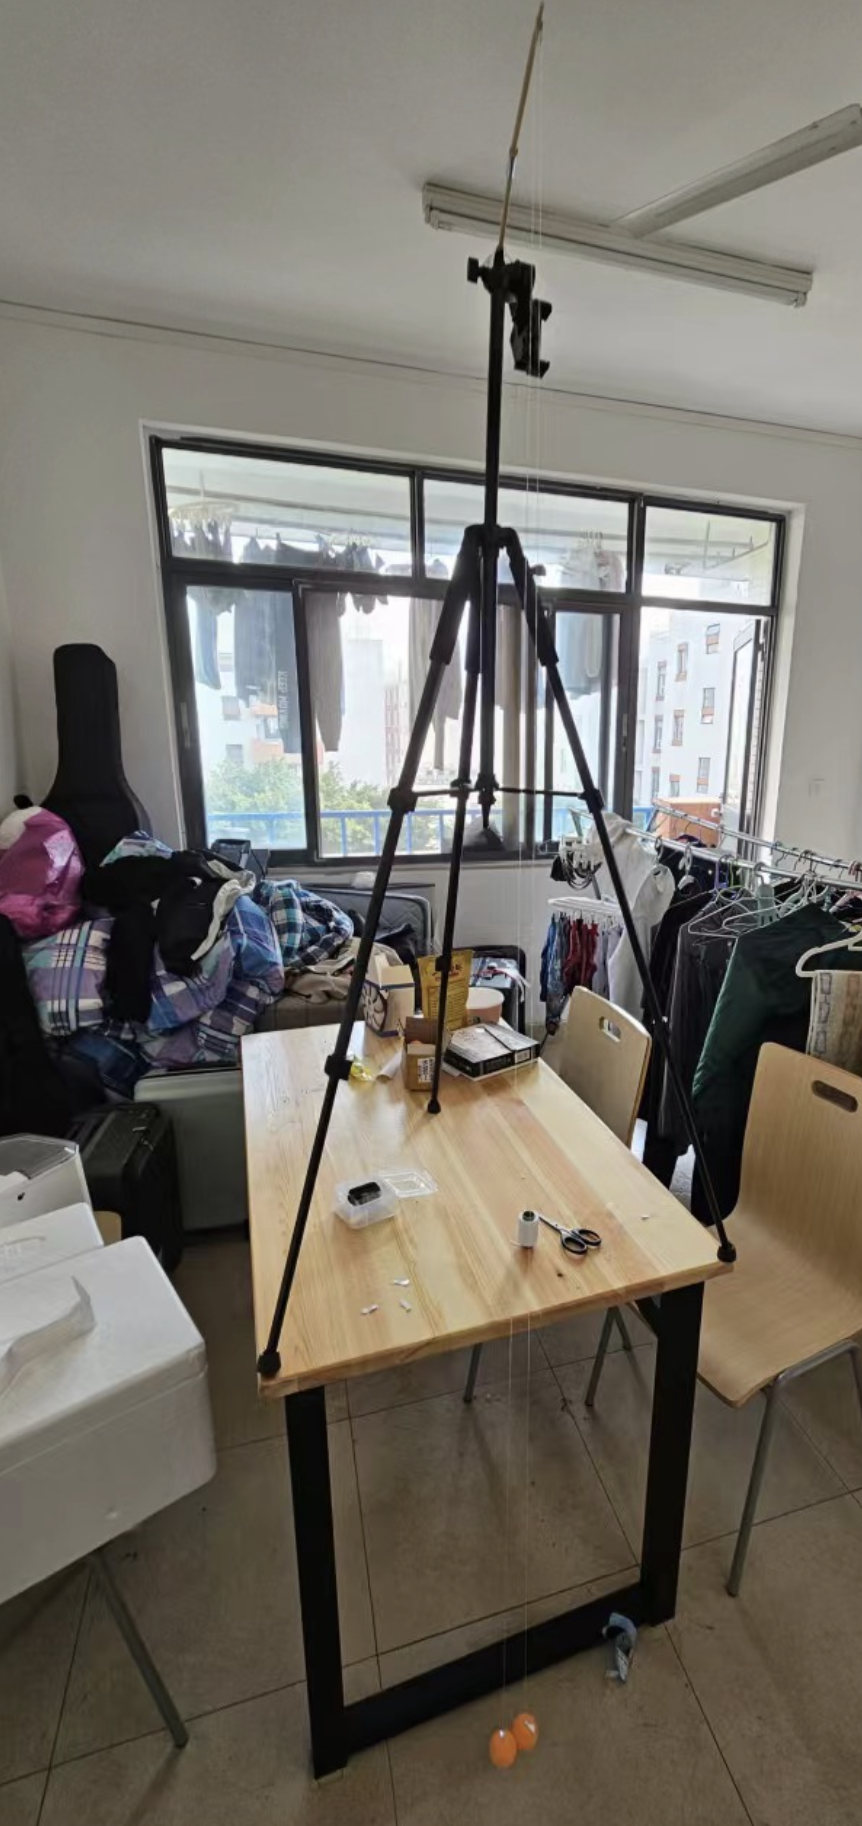
\includegraphics[scale=0.25]{2.png}}
\subfloat[Model Design Diagram.]{
		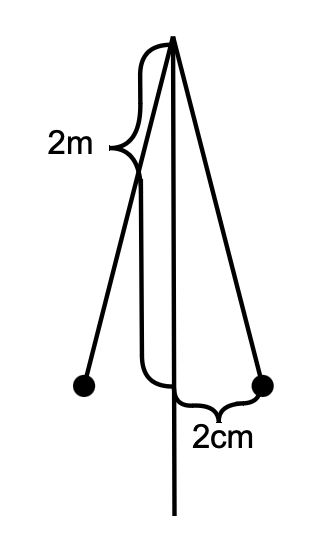
\includegraphics[scale=0.87]{3.png}}
\caption{Structure Diagram.}
\end{figure}

\section{Results}
By researching the parameters of the ping pong ball, we determined that the diameter ($d$) is 4 cm, and the mass ($m$) is 2.7 g. Through measurements, we found that the height($h$) of the platform is 2 m.

Upon modeling and abstraction, it is evident that the distance ($l$) between the centers of the two balls is equal to the diameter ($d$). ($F_s$) represents the tension force in the string, ($F_e$) denotes the Coulomb force, and ($G$) stands for gravity.

\begin{figure}[h]
    \centering
    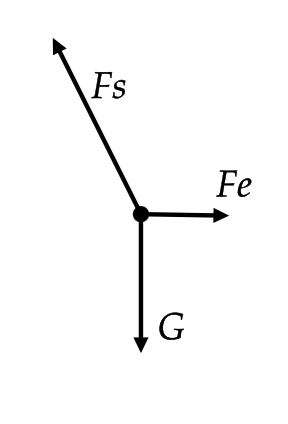
\includegraphics[width=0.3\linewidth]{4.png}
    \caption{Force Analysis.}
\end{figure}

See, Figure 3, we can have
$$
\tan{\theta} = \frac{r}{h} = \frac{F_e}G 
$$
$$
F_e = mg\frac{r}h = 2.7\times10^{-3} \times 9.8 \times \frac{0.02}{2}\text{N}=0.0002646\text{N}.
$$

According to Coulomb's Law, we can deduce that
$$
F_e = \frac{kQq}{l^2} = \frac{kq^2}{l^2} 
$$
$$
q = \sqrt{\frac{F_el^2}{k}} = \sqrt{\frac{0.0002646\times0.04^2}{8.98755 \times 10^{9}}} \text{C}= 6.86332\times 10^{-9}\text{C}
$$

After just experiencing friction and before any charge separation, the individual charge of a single ping pong ball is
$$
q_{initial} = 2q = 1.372664\times 10^{-8}
$$




\section{Discussion}
\label{sec:con}
In this experiment, we initially used a single tripod to measure the angle formed by suspending two friction-charged ocean balls. During the actual experiment, we found that the charge on the balls was not sufficient to separate them. As a solution, we decided to combine the table and the tripod to create a higher platform. This allowed for a smaller Coulomb force to produce a visible angle. However, even with this setup, there was still no observable angle. Finally, we employed smaller diameter ping pong balls, which successfully achieved the desired effect. The advantage of this experiment lies in the use of a higher platform and smaller diameter ping pong balls.

\end{document} 